% Options for packages loaded elsewhere
\PassOptionsToPackage{unicode}{hyperref}
\PassOptionsToPackage{hyphens}{url}
\PassOptionsToPackage{dvipsnames,svgnames,x11names}{xcolor}
%
\documentclass[
  letterpaper,
  DIV=11,
  numbers=noendperiod]{scrartcl}

\usepackage{amsmath,amssymb}
\usepackage{iftex}
\ifPDFTeX
  \usepackage[T1]{fontenc}
  \usepackage[utf8]{inputenc}
  \usepackage{textcomp} % provide euro and other symbols
\else % if luatex or xetex
  \usepackage{unicode-math}
  \defaultfontfeatures{Scale=MatchLowercase}
  \defaultfontfeatures[\rmfamily]{Ligatures=TeX,Scale=1}
\fi
\usepackage{lmodern}
\ifPDFTeX\else  
    % xetex/luatex font selection
    \setmainfont[]{Times New Roman}
\fi
% Use upquote if available, for straight quotes in verbatim environments
\IfFileExists{upquote.sty}{\usepackage{upquote}}{}
\IfFileExists{microtype.sty}{% use microtype if available
  \usepackage[]{microtype}
  \UseMicrotypeSet[protrusion]{basicmath} % disable protrusion for tt fonts
}{}
\makeatletter
\@ifundefined{KOMAClassName}{% if non-KOMA class
  \IfFileExists{parskip.sty}{%
    \usepackage{parskip}
  }{% else
    \setlength{\parindent}{0pt}
    \setlength{\parskip}{6pt plus 2pt minus 1pt}}
}{% if KOMA class
  \KOMAoptions{parskip=half}}
\makeatother
\usepackage{xcolor}
\setlength{\emergencystretch}{3em} % prevent overfull lines
\setcounter{secnumdepth}{5}
% Make \paragraph and \subparagraph free-standing
\makeatletter
\ifx\paragraph\undefined\else
  \let\oldparagraph\paragraph
  \renewcommand{\paragraph}{
    \@ifstar
      \xxxParagraphStar
      \xxxParagraphNoStar
  }
  \newcommand{\xxxParagraphStar}[1]{\oldparagraph*{#1}\mbox{}}
  \newcommand{\xxxParagraphNoStar}[1]{\oldparagraph{#1}\mbox{}}
\fi
\ifx\subparagraph\undefined\else
  \let\oldsubparagraph\subparagraph
  \renewcommand{\subparagraph}{
    \@ifstar
      \xxxSubParagraphStar
      \xxxSubParagraphNoStar
  }
  \newcommand{\xxxSubParagraphStar}[1]{\oldsubparagraph*{#1}\mbox{}}
  \newcommand{\xxxSubParagraphNoStar}[1]{\oldsubparagraph{#1}\mbox{}}
\fi
\makeatother


\providecommand{\tightlist}{%
  \setlength{\itemsep}{0pt}\setlength{\parskip}{0pt}}\usepackage{longtable,booktabs,array}
\usepackage{calc} % for calculating minipage widths
% Correct order of tables after \paragraph or \subparagraph
\usepackage{etoolbox}
\makeatletter
\patchcmd\longtable{\par}{\if@noskipsec\mbox{}\fi\par}{}{}
\makeatother
% Allow footnotes in longtable head/foot
\IfFileExists{footnotehyper.sty}{\usepackage{footnotehyper}}{\usepackage{footnote}}
\makesavenoteenv{longtable}
\usepackage{graphicx}
\makeatletter
\def\maxwidth{\ifdim\Gin@nat@width>\linewidth\linewidth\else\Gin@nat@width\fi}
\def\maxheight{\ifdim\Gin@nat@height>\textheight\textheight\else\Gin@nat@height\fi}
\makeatother
% Scale images if necessary, so that they will not overflow the page
% margins by default, and it is still possible to overwrite the defaults
% using explicit options in \includegraphics[width, height, ...]{}
\setkeys{Gin}{width=\maxwidth,height=\maxheight,keepaspectratio}
% Set default figure placement to htbp
\makeatletter
\def\fps@figure{htbp}
\makeatother

\KOMAoption{captions}{tableheading}
\makeatletter
\@ifpackageloaded{caption}{}{\usepackage{caption}}
\AtBeginDocument{%
\ifdefined\contentsname
  \renewcommand*\contentsname{Table of contents}
\else
  \newcommand\contentsname{Table of contents}
\fi
\ifdefined\listfigurename
  \renewcommand*\listfigurename{List of Figures}
\else
  \newcommand\listfigurename{List of Figures}
\fi
\ifdefined\listtablename
  \renewcommand*\listtablename{List of Tables}
\else
  \newcommand\listtablename{List of Tables}
\fi
\ifdefined\figurename
  \renewcommand*\figurename{Figure}
\else
  \newcommand\figurename{Figure}
\fi
\ifdefined\tablename
  \renewcommand*\tablename{Table}
\else
  \newcommand\tablename{Table}
\fi
}
\@ifpackageloaded{float}{}{\usepackage{float}}
\floatstyle{ruled}
\@ifundefined{c@chapter}{\newfloat{codelisting}{h}{lop}}{\newfloat{codelisting}{h}{lop}[chapter]}
\floatname{codelisting}{Listing}
\newcommand*\listoflistings{\listof{codelisting}{List of Listings}}
\makeatother
\makeatletter
\makeatother
\makeatletter
\@ifpackageloaded{caption}{}{\usepackage{caption}}
\@ifpackageloaded{subcaption}{}{\usepackage{subcaption}}
\makeatother

\ifLuaTeX
  \usepackage{selnolig}  % disable illegal ligatures
\fi
\usepackage{bookmark}

\IfFileExists{xurl.sty}{\usepackage{xurl}}{} % add URL line breaks if available
\urlstyle{same} % disable monospaced font for URLs
\hypersetup{
  pdftitle={Tifosi Bank's Hidden Risk: A Predictive Approach to Customer Churn},
  pdfauthor={Jinyi Tzeng 47969938},
  colorlinks=true,
  linkcolor={blue},
  filecolor={Maroon},
  citecolor={Blue},
  urlcolor={Blue},
  pdfcreator={LaTeX via pandoc}}


\title{Tifosi Bank's Hidden Risk: A Predictive Approach to Customer
Churn}
\usepackage{etoolbox}
\makeatletter
\providecommand{\subtitle}[1]{% add subtitle to \maketitle
  \apptocmd{\@title}{\par {\large #1 \par}}{}{}
}
\makeatother
\subtitle{Machine Learning Insights to Drive Retention}
\author{Jinyi Tzeng 47969938}
\date{}

\begin{document}
\maketitle


\newpage

\section{Executive Summary}\label{executive-summary}

For financial institutions like Tifosi Bank, customers are among the
most valuable assets. Reducing customer attrition has long been a
strategic priority, as every lost customer not only translates to
immediate revenue loss but also diminishes future growth opportunities.
Moreover, acquiring new customers is often significantly more expensive
than retaining existing ones. In this context, establishing a robust
churn prediction and analysis framework is essential for strengthening
the bank's competitive edge.

This study applies machine learning techniques to analyse customer churn
risk using Tifosi Bank's credit card customer dataset. By developing a
suite of classification models---including Logistic Regression,
Ridge/Lasso, Elastic Net, KNN, Random Forest, and XGBoost---we
systematically explored the relationship between customer
characteristics and attrition behaviour.

Model performance was evaluated using multiple metrics. XGBoost clearly
outperformed all other models and emerged as the optimal classifier due
to its superiority across three key dimensions:

\begin{itemize}
\tightlist
\item
  \textbf{Generalisation}: Achieved a ROC AUC of 0.996, indicating
  strong discriminative power on unseen data.
\item
  \textbf{Precision}: Reached 0.984, reducing false positives and
  limiting unnecessary retention costs for high-value customers.
\item
  \textbf{Recall}: Attained 0.990, ensuring that nearly all churned
  customers were correctly identified.
\end{itemize}

Recognising the inherent trade-off between precision and recall, we
further assessed F1 Score (0.987) to validate XGBoost's ability to
maintain a strong balance between these two goals. Based on this
comprehensive evaluation, XGBoost was selected as the best-performing
model for this analysis.

Based on the model's variable importance analysis, three high-risk
customer segments were identified: (1) customers with declining
transaction frequency, (2) older customers and those with high credit
limits, and (3) customers with frequent contact with customer service.

We recommend Tifosi Bank take the following actions:\\
-- \textbf{Re-engagement campaigns} for low-activity customers through
cashback offers, reminder emails, or limited-time promotions. For
instance, JPMorgan Chase's email reactivation campaigns showed a 12\%
re-engagement rate in similar segments (Forrester, 2023).\\
-- \textbf{Tailored retention offers} for older or high-credit
customers, such as personalised interest reviews, loyalty perks, or
bundled financial products, which have been shown to improve customer
stickiness in senior segments (Deloitte, 2021).\\
-- \textbf{Service quality improvements} for frequent callers by
flagging them for proactive support and routing them to experienced
agents. Citibank's churn-risk scoring includes service logs as a key
input for customer dissatisfaction (IBM, 2020).

These strategies enable Tifosi Bank to move from reactive churn
mitigation to a proactive, data-driven retention approach.

\section{Introduction \& Business
Context}\label{introduction-business-context}

Credit card churn poses a significant threat to the profitability,
customer lifetime value, and strategic growth of retail banks. With
credit card operations contributing up to 25\% of a bank's retail
revenue---driven by interest income, interchange fees, annual charges,
and cross-selling opportunities (McKinsey, 2023)---a rising churn rate
represents not just a revenue loss but a potential erosion of customer
trust and competitive positioning.

For Tifosi Bank, a recent spike in credit card attrition raises concerns
about declining engagement and highlights the need for timely
intervention. Left unaddressed, this trend may increase acquisition
costs, weaken cross-sell pipelines, and undermine long-term market
share. Identifying high-risk segments and understanding the key
behavioral or demographic drivers of churn is essential to enable
targeted, cost-effective retention strategies.

This report applies predictive modeling techniques to develop a churn
classification framework tailored to Tifosi Bank's credit card
portfolio. By leveraging machine learning on behavioral and demographic
data, we aim to provide actionable insights that inform retention
planning, resource allocation, and customer experience
management---ultimately helping leadership mitigate risk and sustain
growth in a highly competitive market.

\section{Analytical Overview}\label{analytical-overview}

\subsection{Dataset Summary}\label{dataset-summary}

The dataset from Tifosi Bank consists of 10,127 credit card customers,
each represented by a range of 21 variables across three main feature
groups: -- Demographic information (e.g., age, income, education level)
-- Behavioural indicators (e.g., transaction amounts, credit usage
ratios) -- Account relationship metrics (e.g., months on book, number of
products held)

The target variable, Attrition\_Flag, is a binary indicator of customer
status, where ``Attrited Customer'' denotes churn and ``Existing
Customer'' indicates retention. The dataset is imbalanced, with only
around 16\% of customers having churned, which presents additional
considerations when building predictive models.

\newpage

Table 1. Representative Variables by Group

\begin{center}
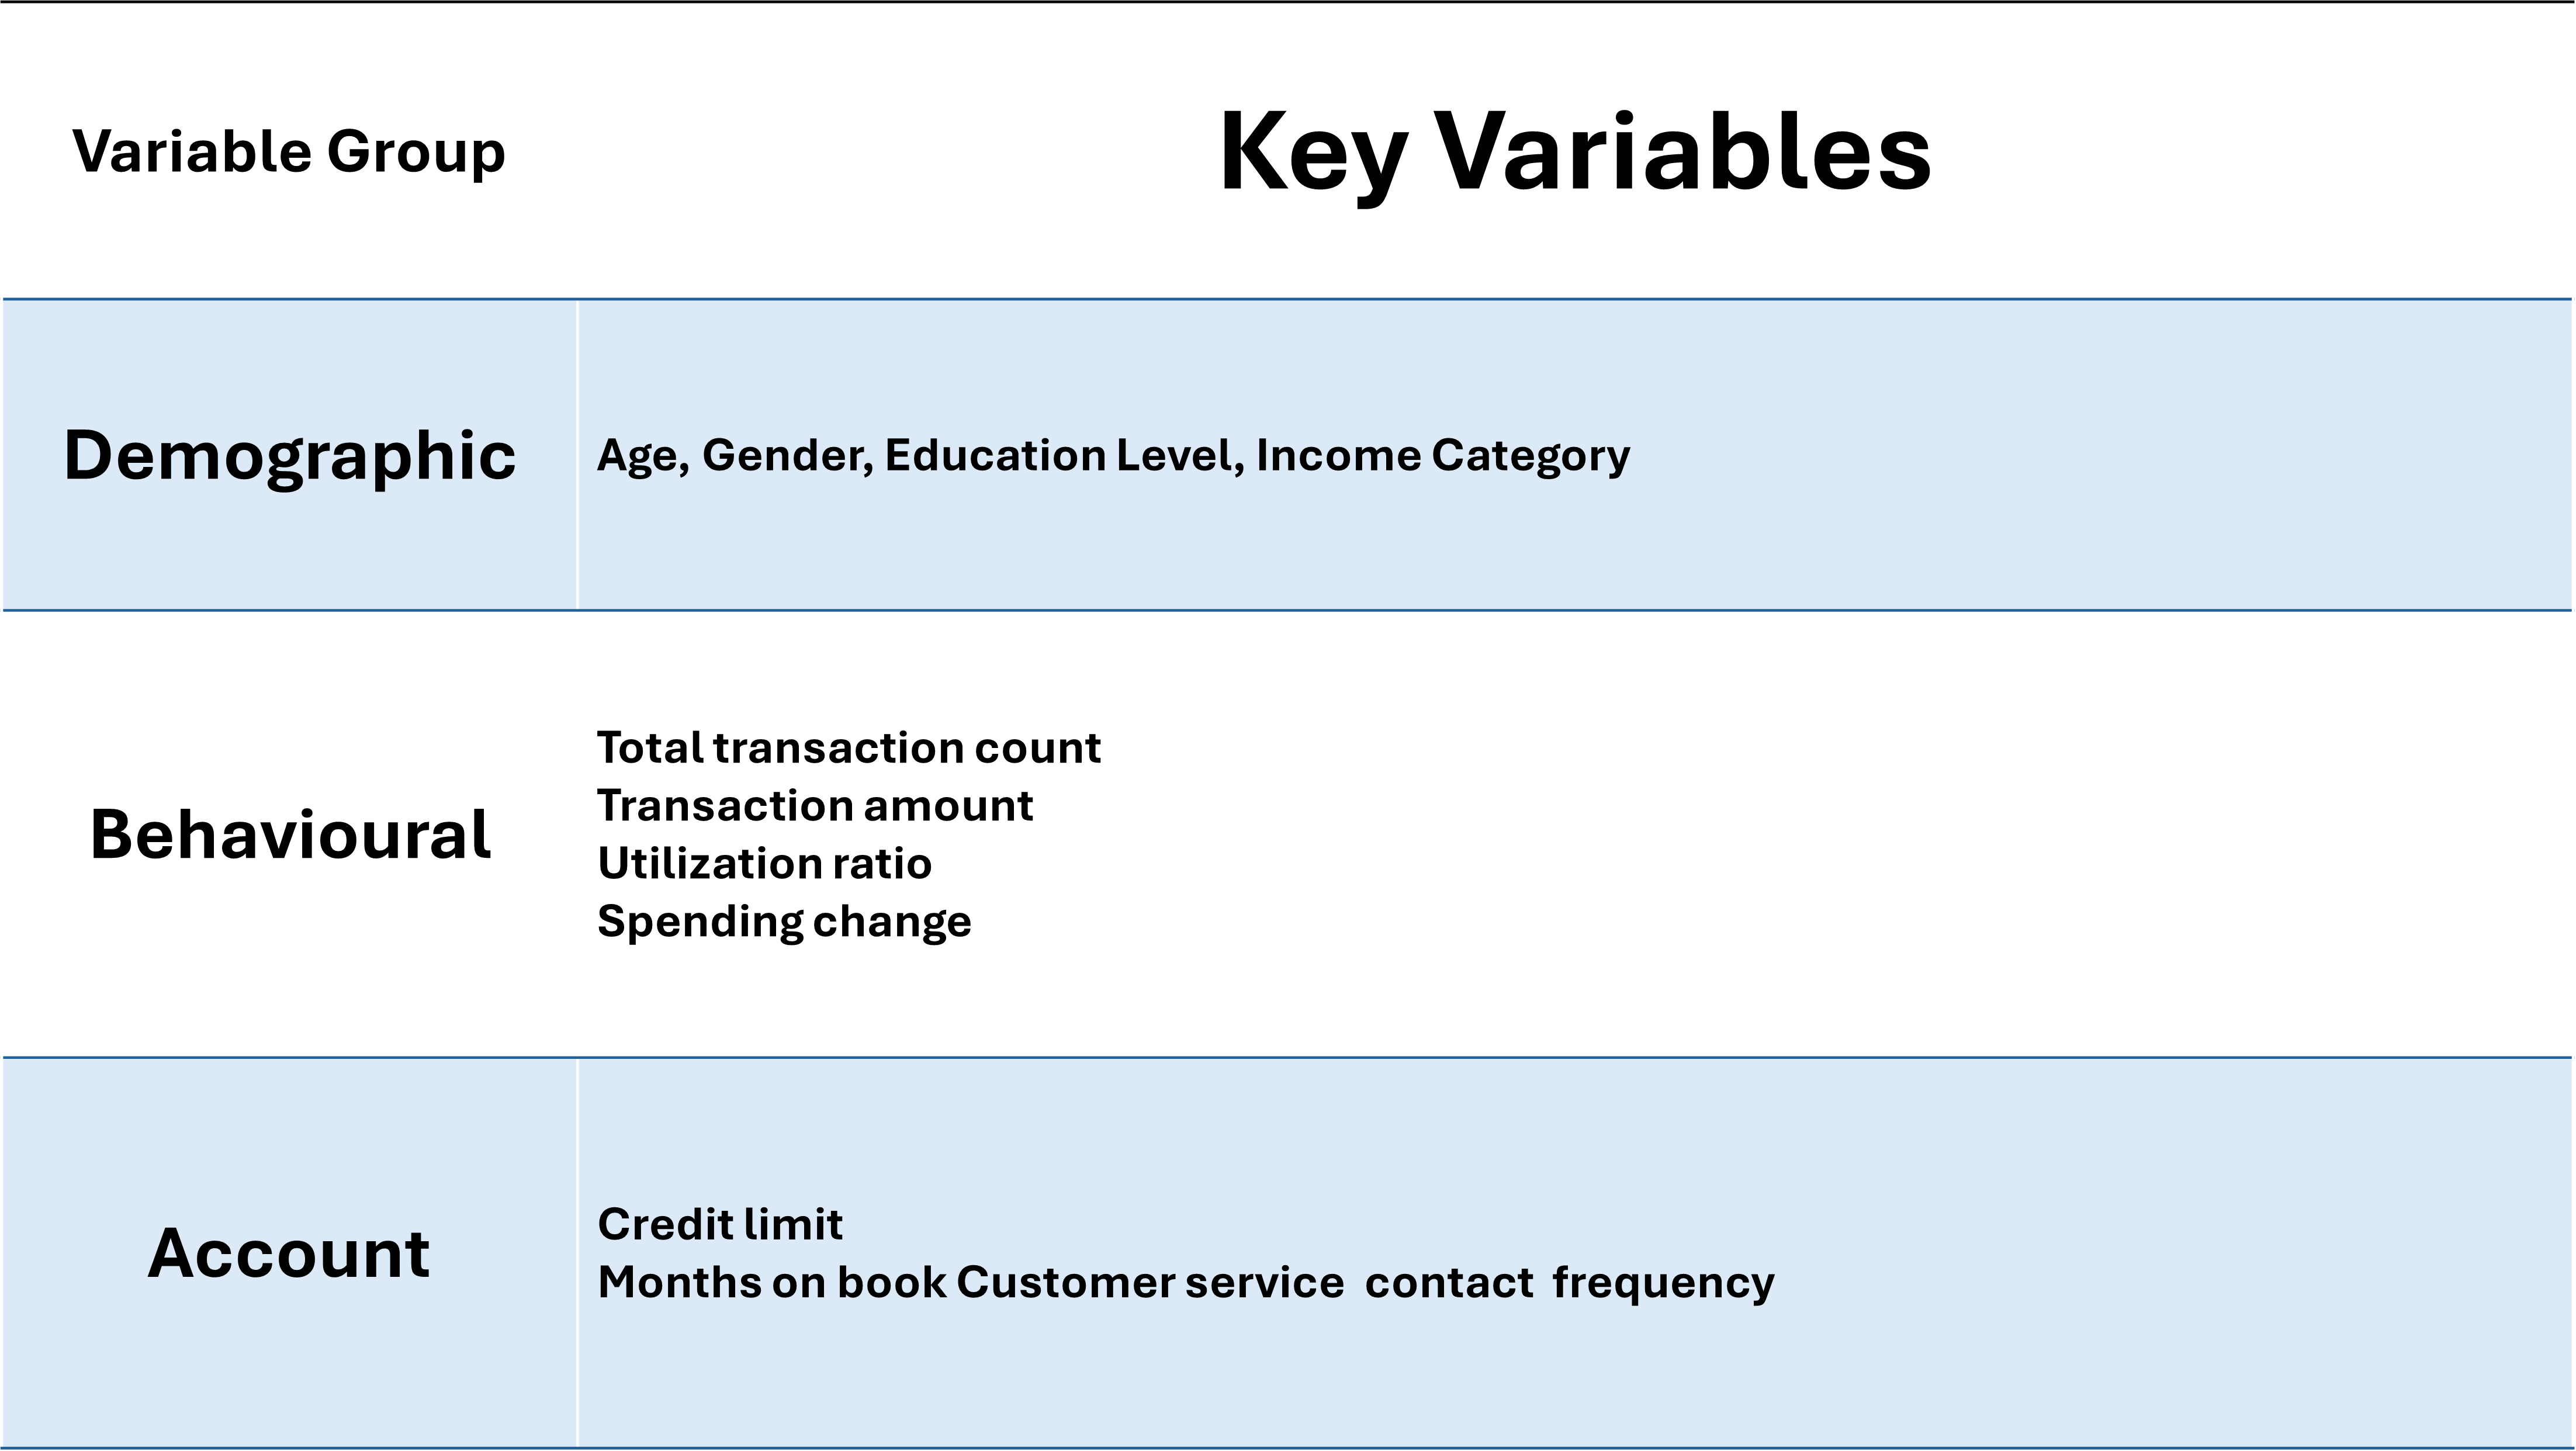
\includegraphics{figures/key_variables_summary.png}
\end{center}

Note: This table only shows representative variables from each category.
Full feature set used in modeling.

\newpage

\subsection{Exploratory View}\label{exploratory-view}

\subsubsection{Churn rate is crucial}\label{churn-rate-is-crucial}

Only 16.1\% of customers have churned, revealing a highly imbalanced
dataset. This reinforces the importance of using appropriate evaluation
metrics---such as ROC AUC and recall---that are less sensitive to
imbalance than accuracy alone.

\begin{center}
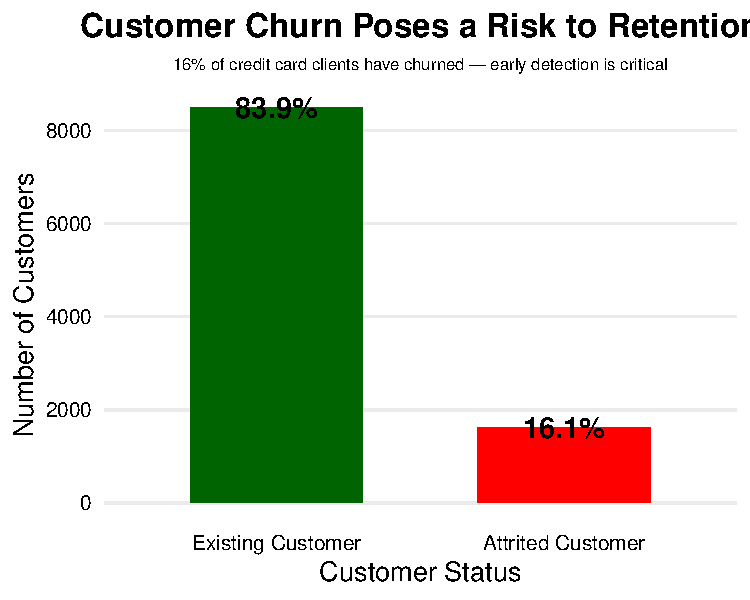
\includegraphics[width=0.8\textwidth,height=\textheight]{v4_files/figure-pdf/unnamed-chunk-14-1.pdf}
\end{center}

\subsubsection{Total transaction count shows more
evidence}\label{total-transaction-count-shows-more-evidence}

Customers who churned exhibit markedly fewer transactions over the past
year. The median transaction count is significantly lower compared to
retained customers, and the distribution is more compressed. This
confirms transactional activity as a key behavioral indicator of churn.

\begin{center}
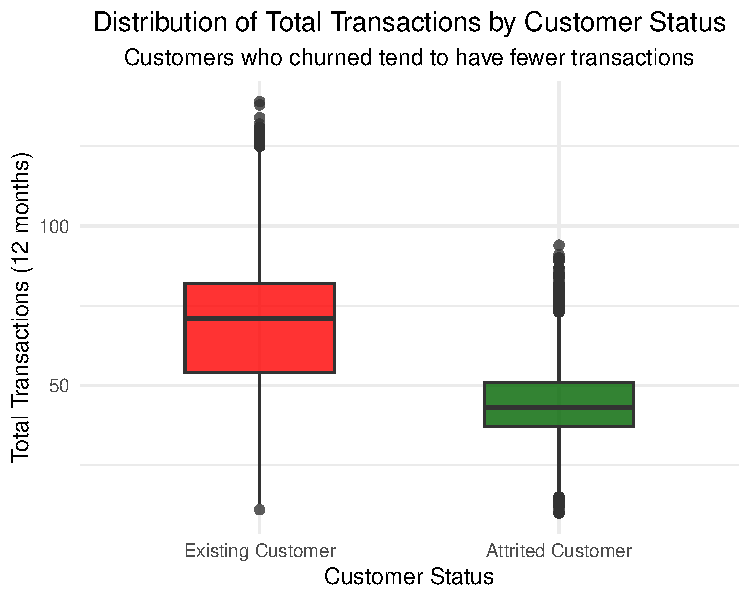
\includegraphics[width=0.8\textwidth,height=\textheight]{v4_files/figure-pdf/unnamed-chunk-15-1.pdf}
\end{center}

\subsection{Analyzing Workflow
Summary}\label{analyzing-workflow-summary}

To predict customer attrition at Tifosi Bank, we implemented a
structured modelling workflow comprising data preparation, feature
engineering, model development, and performance evaluation. The raw
dataset was first cleaned and preprocessed by removing irrelevant
identifiers, converting character variables to factors, and splitting
the data into training and testing sets.

Key preprocessing steps included encoding categorical variables,
removing near-zero variance and highly correlated predictors, and
standardising numerical features. To account for model-specific
requirements, we constructed tailored preprocessing pipelines (recipes)
for each algorithm. To ensure model generalisability, we employed
10-fold cross-validation on the training data, stratified by churn
status.

We developed and tuned a range of classification models, including
baseline logistic regression, regularised models (ridge, lasso, elastic
net), k-nearest neighbors (KNN), random forest, and extreme gradient
boosting (XGBoost). Each model was tuned using grid search to optimise
key hyperparameters, and performance was evaluated using ROC AUC,
precision, recall, accuracy, and F1 score.

After identifying the best-performing models through cross-validation,
we retrained them on the full training set and assessed their predictive
performance on the test set. This end-to-end workflow allowed for both
accurate prediction and insightful comparison across modelling
approaches.

\begin{figure}[H]

{\centering 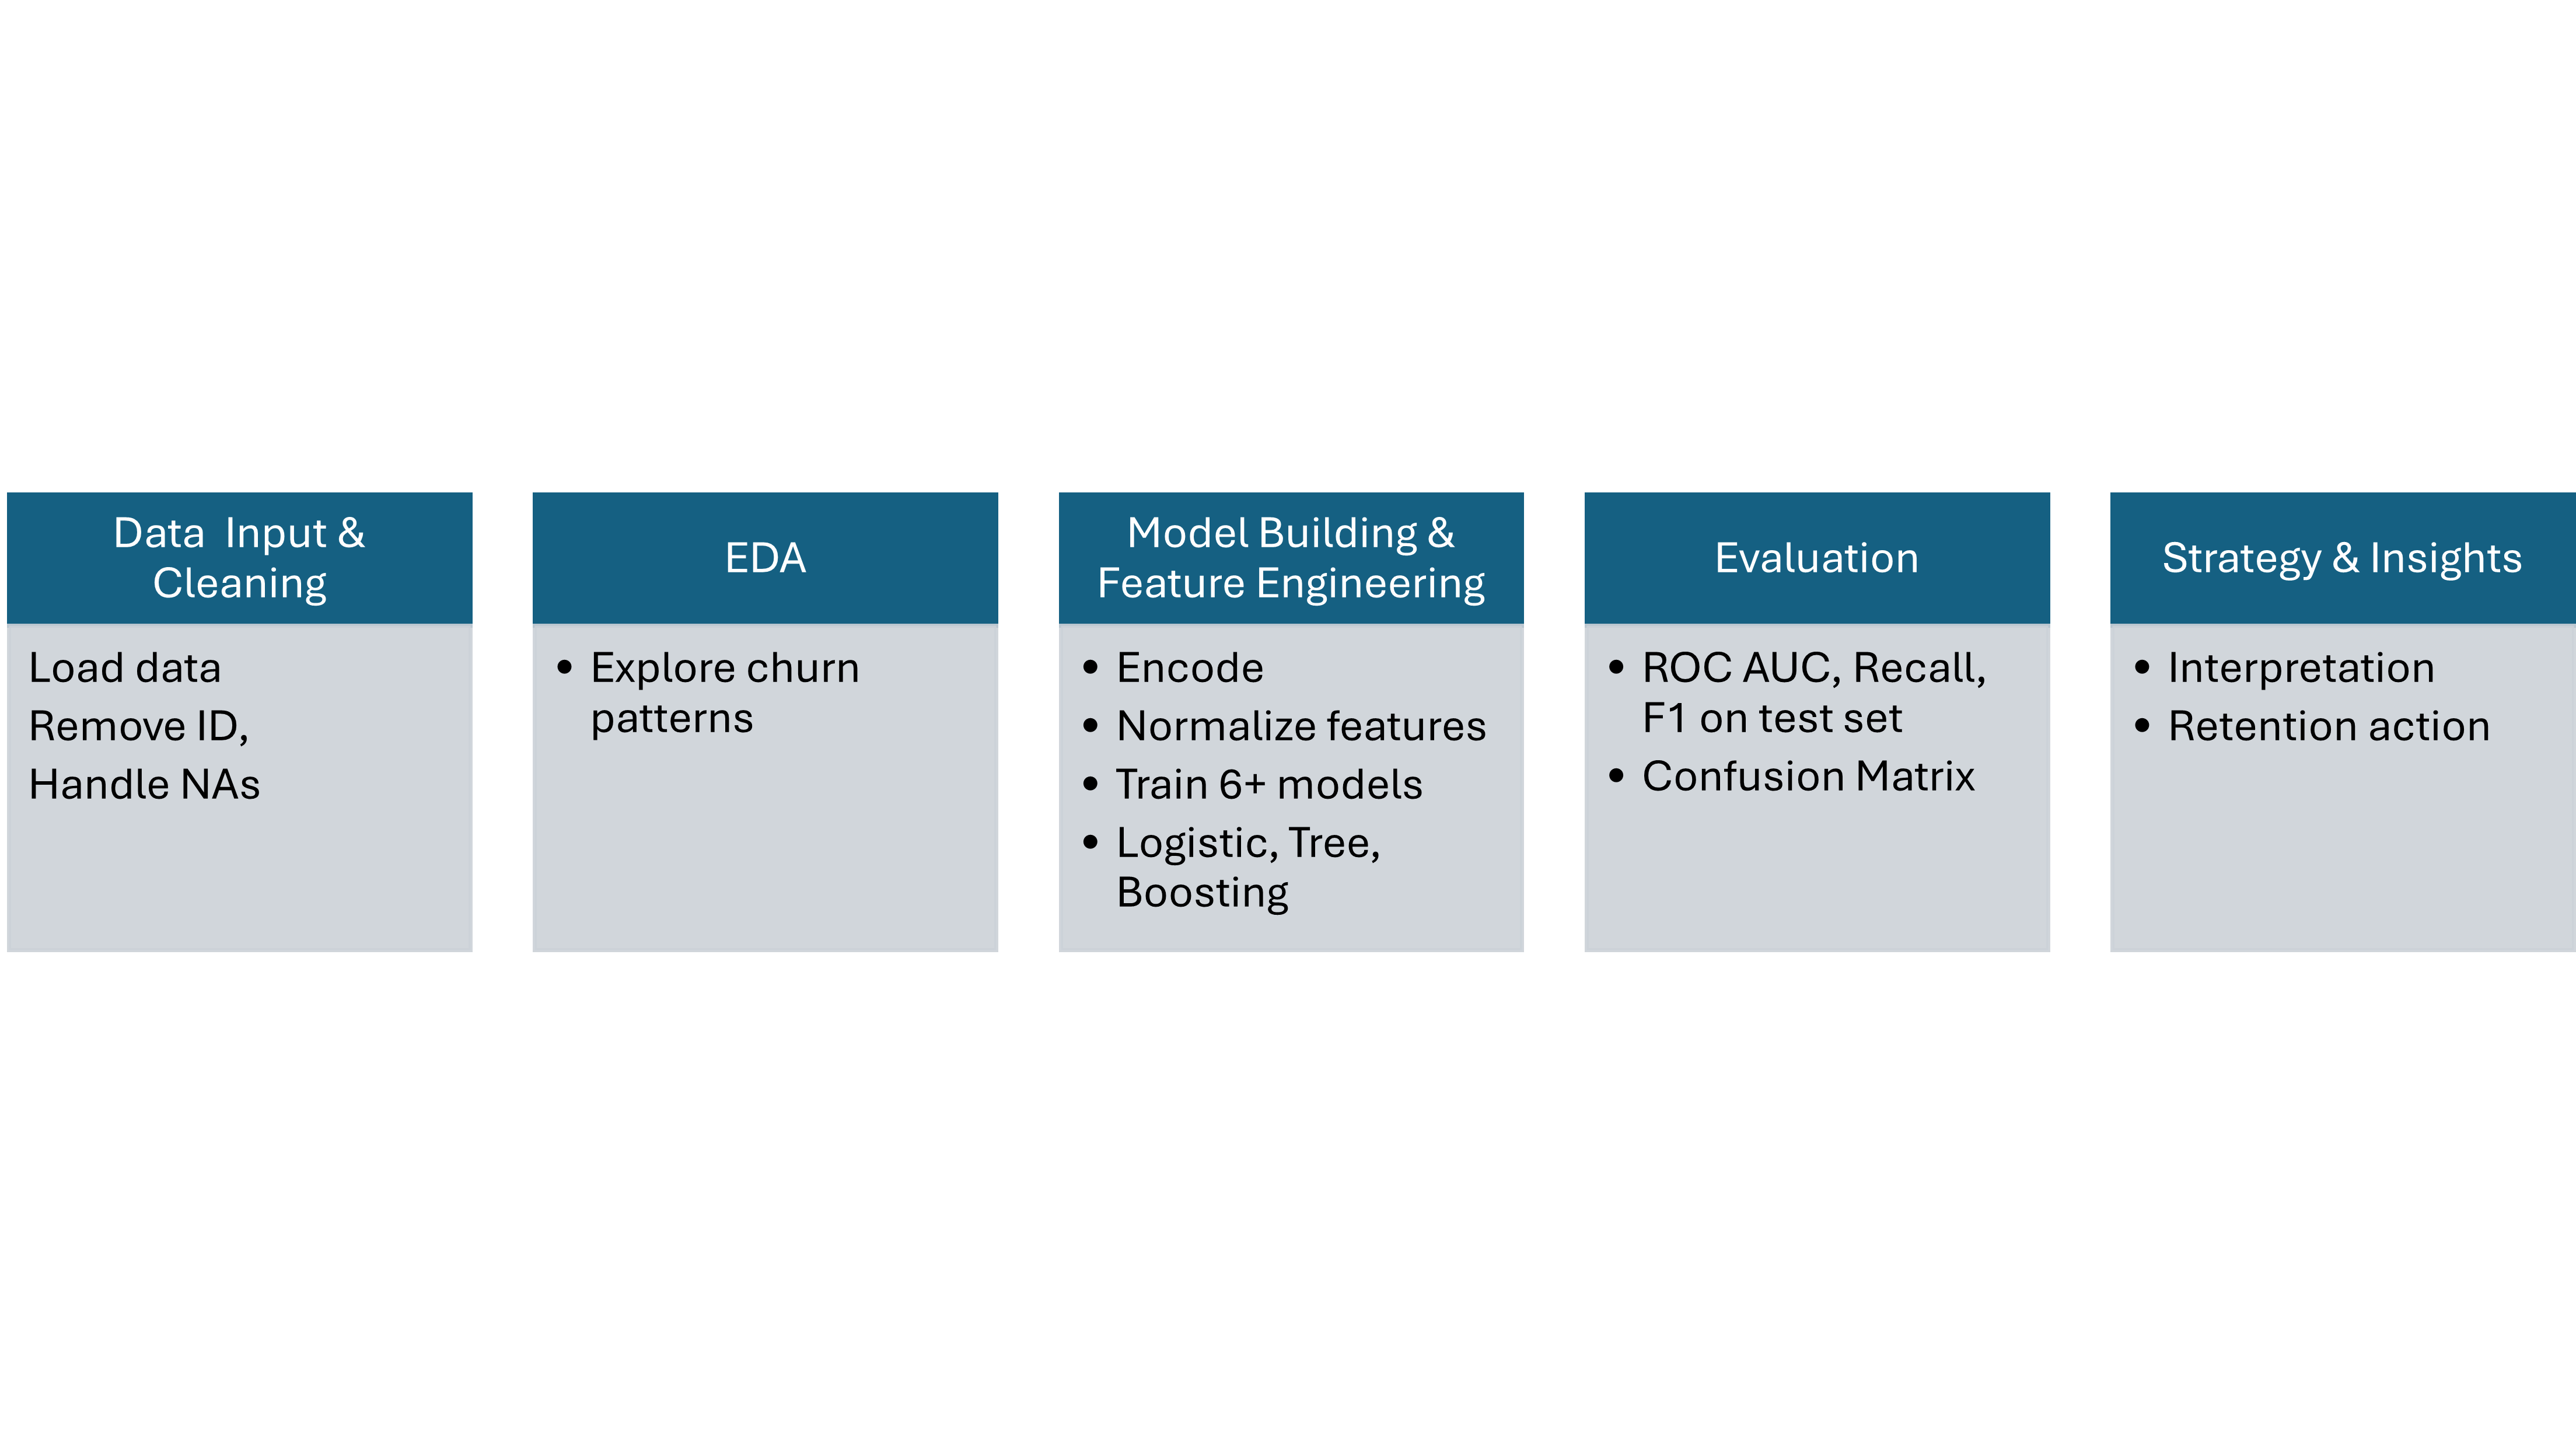
\includegraphics[width=0.85\textwidth,height=\textheight]{Output/Workflow Overview.png}

}

\caption{Workflow Overview}

\end{figure}%

\subsection{Why This Approach ?}\label{why-this-approach}

Given the high stakes of customer churn, a robust predictive strategy
was necessary. Rather than relying on a single model, we employed
multiple algorithms to compare performance across different assumptions
and learning styles. This approach ensures reliability, maximises
predictive accuracy, and provides interpretable outputs for business
decision-making.

\newpage

\section{Key Insights \& Visual
Storytelling}\label{key-insights-visual-storytelling}

\subsection{Model Performance
Comparison}\label{model-performance-comparison}

To identify the most effective model for churn prediction, we compared
seven classification algorithms across five evaluation metrics:
accuracy, recall, precision, F1 score, and area under the ROC curve
(AUC). Table 1 presents the performance summary on the hold-out test
set.

Overall, XGBoost emerged as the top-performing model, achieving the
highest scores across all metrics. It attained an accuracy of 0.978, a
recall of 0.990, and a precision of 0.984, leading to an F1 score of
0.987 and an AUC of 0.996. These results indicate exceptional
discriminative power and balance between false positives and false
negatives.

Random Forest also demonstrated strong performance, with a recall of
0.992 and an F1 score of 0.979. However, its precision and AUC remained
slightly below that of XGBoost. Among the simpler models, logistic
regression and its regularised variants (ridge, lasso, elastic net)
performed consistently but less competitively, with AUC values around
0.931. KNN achieved the highest recall among non-tree-based models
(0.987) but showed lower precision and AUC.

These comparisons provided a robust justification for selecting XGBoost
as the final model for churn classification.

\begin{longtable}[]{@{}llllll@{}}
\toprule\noalign{}
Model & Accuracy & Recall & Precision & F1 Score & ROC AUC \\
\midrule\noalign{}
\endhead
\bottomrule\noalign{}
\endlastfoot
Logistic & 0.909 & 0.963 & 0.931 & 0.947 & 0.931 \\
Ridge & 0.905 & 0.978 & 0.915 & 0.945 & 0.922 \\
Lasso & 0.909 & 0.963 & 0.931 & 0.947 & 0.931 \\
Elastic Net & 0.909 & 0.963 & 0.931 & 0.947 & 0.931 \\
KNN & 0.901 & 0.987 & 0.904 & 0.943 & 0.926 \\
Random Forest & 0.965 & 0.992 & 0.967 & 0.979 & 0.993 \\
XGBoost & 0.978 & 0.990 & 0.984 & 0.987 & 0.996 \\
\end{longtable}

\subsection{Visual Evaluation}\label{visual-evaluation}

\subsubsection{ROC Curve-Generalisation
ability}\label{roc-curve-generalisation-ability}

The figure presents the ROC curve (Receiver Operating Characteristic)
for the XGBoost model, which evaluates the model's ability to
distinguish between customers who churned and those who remained. A ROC
curve that closely follows the top-left border of the graph indicates a
highly effective model, as it reflects a strong balance between
sensitivity (true positive rate) and specificity (false positive rate).
In this case, the curve demonstrates an Area Under the Curve (AUC) value
of 0.996, which is near perfect.

This exceptionally high AUC suggests that the model can almost
flawlessly separate churned customers from those who stay, even when
applied to new, unseen data. Such performance confirms the model's
strong generalisation capacity, which is critical for real-world
deployment. For Tifosi Bank, this means that the model provides a highly
reliable foundation for predicting churn risk and supporting timely,
data-driven retention strategies.

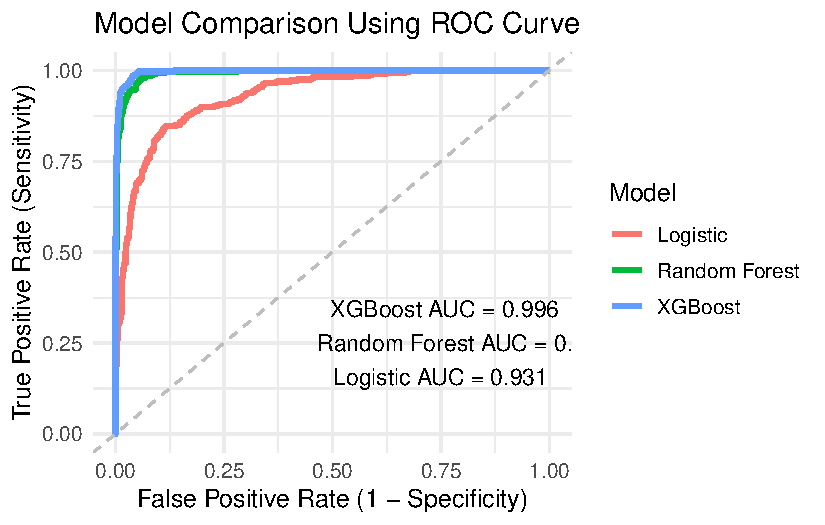
\includegraphics{v4_files/figure-pdf/unnamed-chunk-17-1.pdf}

\subsubsection{Confusion Matrix-who it predicts correctly, and where it
misfires}\label{confusion-matrix-who-it-predicts-correctly-and-where-it-misfires}

The confusion matrix illustrates that the XGBoost model demonstrates
strong predictive performance at a threshold of 0.5, correctly
classifying 1,982 out of 2,026 customers. The breakdown is as follows:

True Positives (TP = 299): Customers who actually churned and were
correctly identified by the model. These customers represent actionable
cases where proactive retention strategies could be applied to prevent
revenue loss.

True Negatives (TN = 1,683): Customers who stayed and were accurately
predicted as such. Correctly identifying loyal customers allows the bank
to avoid unnecessary retention efforts and focus resources efficiently.

False Positives (FP = 17): Customers who were incorrectly predicted to
churn but actually stayed. While these cases may result in slightly
redundant outreach, they pose minimal business risk and may even improve
customer engagement.

False Negatives (FN = 27): Customers who churned but were missed by the
model. These represent missed intervention opportunities and are the
most critical from a risk management standpoint.

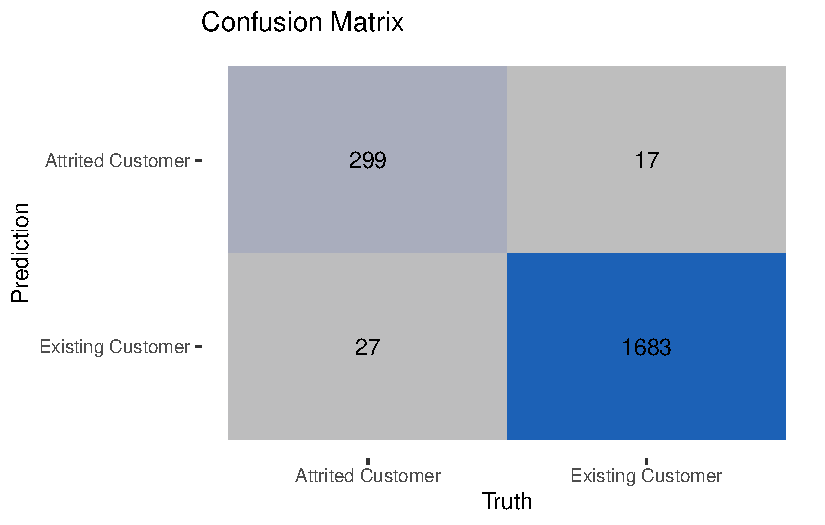
\includegraphics{v4_files/figure-pdf/unnamed-chunk-18-1.pdf}

\subsection{Key Factors of Churn}\label{key-factors-of-churn}

To gain insight into the drivers of customer attrition, we analysed the
variable importance rankings produced by the XGBoost model. As shown in
Figure 4, behavioural features dominated the top positions, highlighting
the strong predictive power of customer activity patterns over
demographic traits.

The most influential variable was \textbf{total transaction count}, with
churned customers exhibiting significantly fewer transactions compared
to retained ones. This was followed by \textbf{total transaction
amount}, reinforcing the role of spending engagement as a key churn
indicator. The third-ranked predictor, \textbf{total revolving balance},
suggests that customers carrying higher outstanding balances may be more
prone to disengagement or financial stress.

Additionally, \textbf{change in transaction count between Q4 and Q1}
emerged as a high-impact dynamic variable, signalling that a recent
decline in activity is a leading indicator of potential churn. The
\textbf{total number of products or relationships held} with the bank
also featured prominently, where lower relationship depth was associated
with higher churn probability.

Interestingly, demographic features such as gender, education level, and
income category had relatively low importance, underscoring the greater
value of behavioural signals in churn prediction.

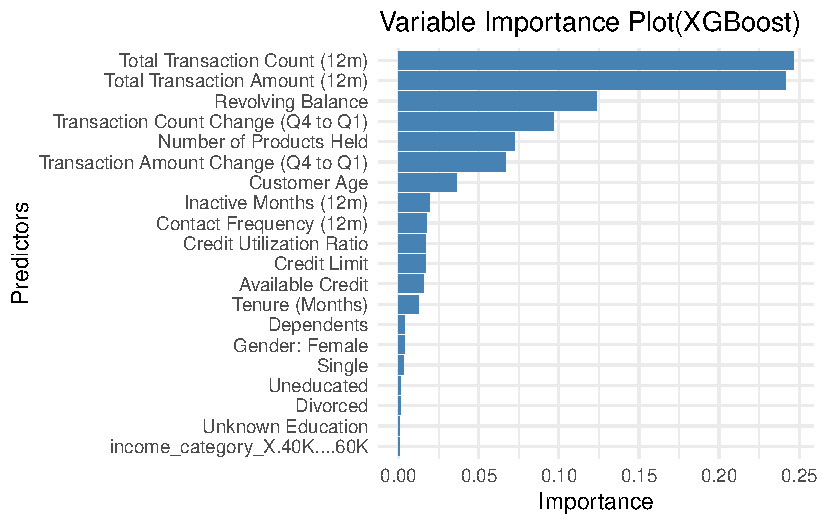
\includegraphics{v4_files/figure-pdf/unnamed-chunk-20-1.pdf}

\subsection{Interpretation \& Strategic
Implications}\label{interpretation-strategic-implications}

The results of the XGBoost model provide several useful insights for
Tifosi Bank's customer retention strategy. The most important factor was
the number of credit card transactions. Customers who made fewer
transactions were much more likely to leave the bank. This means that
low activity can be an early warning sign of churn.

Transaction amount and revolving balance were also strong predictors.
Customers who spent less, or who carried high unpaid balances, showed a
higher chance of leaving. These patterns suggest that both low
engagement and possible financial stress are related to customer
attrition.

A drop in transaction activity compared to the previous quarter was
another key signal. This shows that recent changes in behaviour---not
just overall patterns---can help identify at-risk customers before they
leave.

Lastly, customers with fewer products or weaker relationships with the
bank were more likely to churn. This suggests that increasing
relationship depth (e.g., encouraging them to open savings accounts or
use more services) may help keep customers loyal.

Based on these findings, Tifosi Bank could take action such as: -
\textbf{Monitoring drops in transaction activity} and reaching out early
- \textbf{Offering personalised incentives} to low-activity but
high-limit customers - \textbf{Improving customer support} for those who
contact the bank frequently - \textbf{Encouraging multi-product
relationships} to build loyalty

By using these predictors, the bank can move from reactive to proactive
churn management.

\section{Strategic Implications}\label{strategic-implications}

The XGBoost model highlights three key churn drivers: declining
transaction activity, low spending, and limited product engagement.

\begin{enumerate}
\def\labelenumi{\arabic{enumi}.}
\tightlist
\item
  Low transaction frequency and spend signal disengagement. Tifosi Bank
  should implement monitoring systems to detect early drops in activity.
  Flagged customers can receive timely re-engagement offers---such as
  cashback, reminders, or bundled promotions---to restore value before
  churn occurs.
\end{enumerate}

For example, Bank of America reported a record 23.4 billion digital
interactions in 2023, including proactive spend alerts and personalised
financial guidance, which contributed to stronger customer engagement
across dormant segments (Bank of America, 2024).

\begin{enumerate}
\def\labelenumi{\arabic{enumi}.}
\setcounter{enumi}{1}
\tightlist
\item
  Customers with high revolving balances but low usage may be
  financially stressed or dissatisfied. Targeted support, such as
  usage-based rewards or flexible payment plans, can rebuild trust and
  usage without sacrificing profitability.
\end{enumerate}

Similar strategies are used by Capital One, which emphasises retention
through personalised balance support, loyalty rewards, and credit plan
customisation to address declining engagement in at-risk segments
(Capital One, 2021).

\begin{enumerate}
\def\labelenumi{\arabic{enumi}.}
\setcounter{enumi}{2}
\tightlist
\item
  Customers using multiple bank products are less likely to churn.
  Bundling credit cards with savings, insurance, or loyalty programs can
  deepen relationships and increase switching costs.
\end{enumerate}

A Deloitte insight report noted that banks adopting cross-product
strategies---linking digital channels with core banking services---have
achieved stronger customer retention and lower churn risk (Deloitte,
2025).

\begin{enumerate}
\def\labelenumi{\arabic{enumi}.}
\setcounter{enumi}{3}
\tightlist
\item
  Frequent contact with customer service can signal dissatisfaction.
  Proactively mining service logs and routing high-risk customers to
  trained agents helps turn complaints into retention wins.
\end{enumerate}

IBM's churn classification case study highlights how integrating service
frequency data into predictive models enhances churn flagging accuracy
and allows prioritised human follow-up for high-contact customers (IBM,
2021).

These actions shift Tifosi Bank from reactive churn control to proactive
customer management---boosting customer lifetime value and long-term
profitability.

\begin{figure}[H]

{\centering 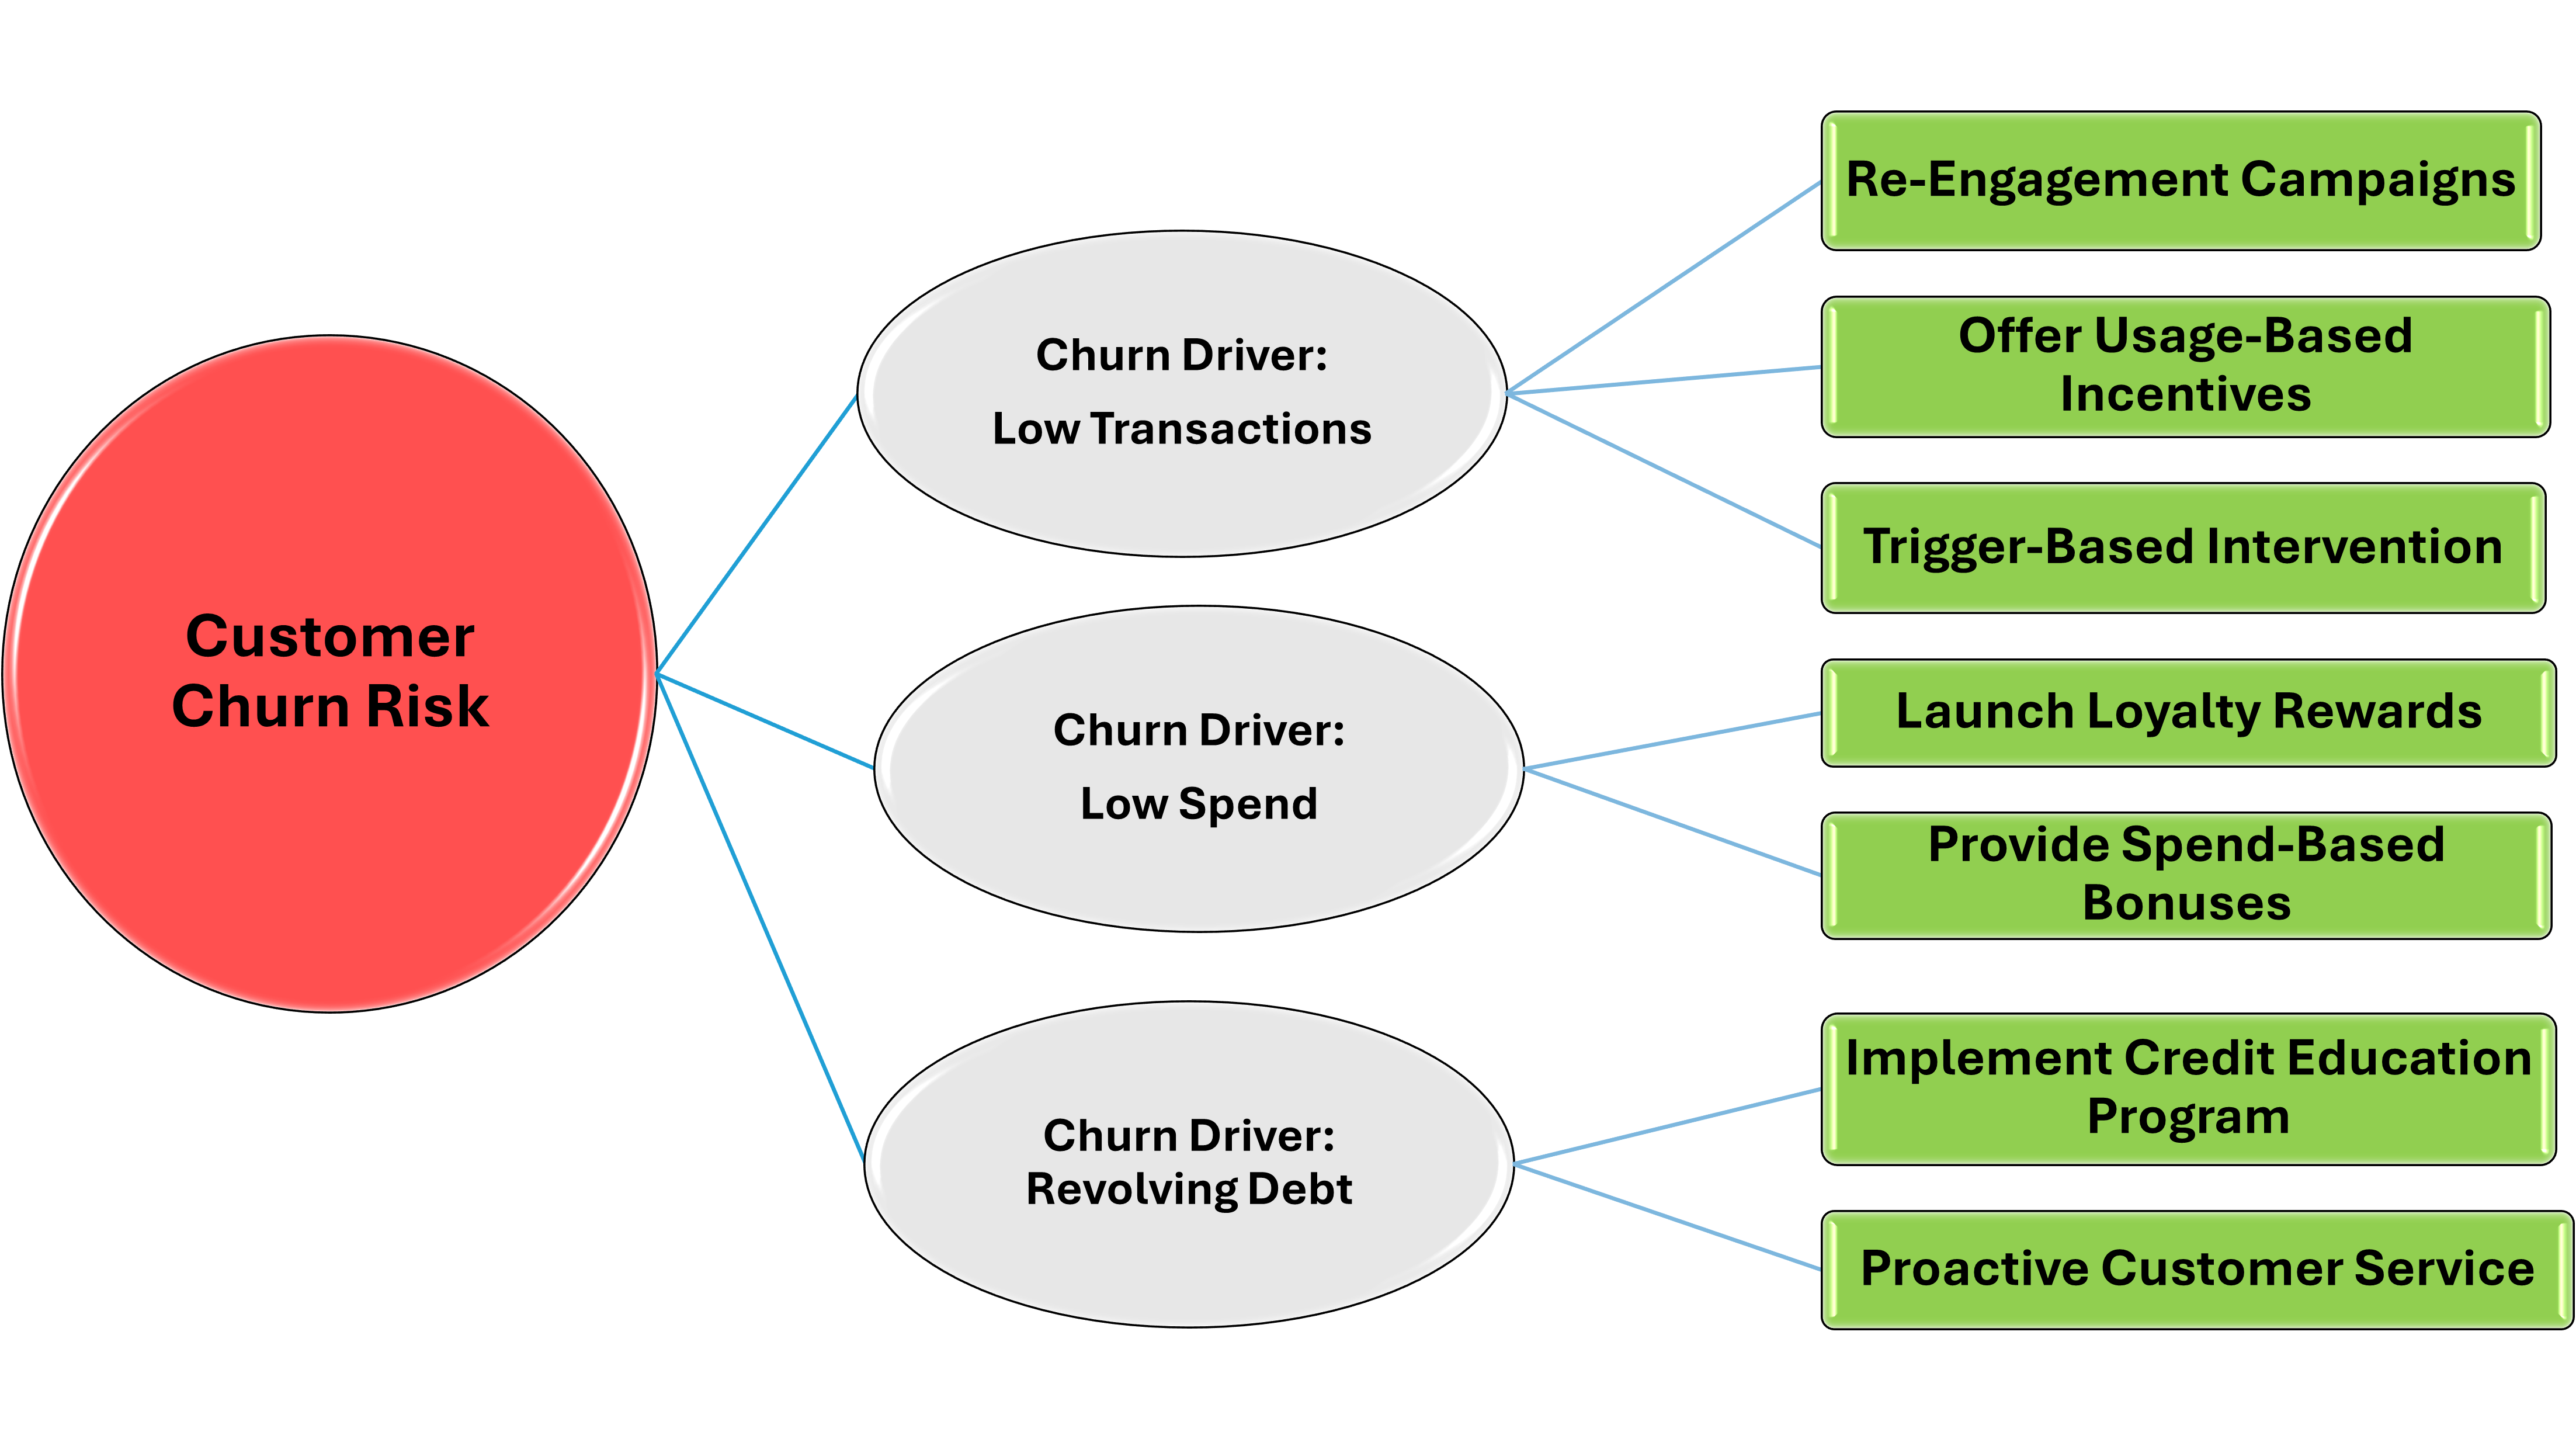
\includegraphics[width=0.85\textwidth,height=\textheight]{figures/strategy01.png}

}

\caption{Churn Strategies}

\end{figure}%

\section{Conclusion and Limitations}\label{conclusion-and-limitations}

This study used machine learning to tackle a key business challenge at
Tifosi Bank: predicting and preventing customer churn. Through a
structured modelling process, XGBoost emerged as the most effective
classifier, driven by strong signals from transaction activity,
engagement depth, and behavioural change.

Beyond technical accuracy, the model's insights offer real business
value. By focusing on declining transactions, low product adoption, and
early dissatisfaction signals, the bank can take targeted action to
retain high-risk customers.

Looking ahead, future work could explore integrating real-time behaviour
tracking and customer feedback into the model. Combining predictive
analytics with human-centred engagement will be key to reducing
attrition and sustaining long-term growth.

In short, understanding who is likely to leave is only half the
battle---the real opportunity lies in knowing what to do before they go.

\newpage

\section{Reference}\label{reference}

Bank of America. (2024). \emph{Digital Engagement Soars at Bank of
America to More Than 10 Billion Logins, up 15\% Year-Over-Year}.

Capital One. (2021). \emph{Customer Loyalty and Retention Strategies}.

Deloitte. (2025). \emph{Retail and Commercial Banking}.

IBM. (2021). \emph{IBM Telco Customer Churn Analysis}.

\begin{center}\rule{0.5\linewidth}{0.5pt}\end{center}




\end{document}
